\begin{enumerate}[label=\thesection.\arabic*.,ref=\thesection.\theenumi]
\numberwithin{equation}{enumi}
\item A unity feedback control system is characterised by the open-loop transfer function
\begin{align}
G(S) = \frac{2(s+1)}{s^3 + ks^2 + 2s +1}
\end{align}
the value of the k for which the system oscillates at 2 rad/s

\solution
Modelling Closed loop system G(s) into a Open loop system Gm(s)

\tikzstyle{block} = [draw, fill=blue!20, rectangle, 
    minimum height=0.7cm, minimum width=0.7cm]
\tikzstyle{sum} = [draw, fill=blue!20, circle, node distance=1cm]
\tikzstyle{input} = [coordinate]
\tikzstyle{output} = [coordinate]
\tikzstyle{pinstyle} = [pin edge={to-,thin,black}]

\begin{tikzpicture}[auto, node distance=2.5cm,>=latex']
    % We start by placing the blocks
    \node [input, name=input] {};
    \node [sum, right of=input] (sum) {};
    \node [block, right of=sum] (controller) {G(s)};
    \node [output, right of=controller] (output) {};
    \node [block, below of=controller] (measurements) {H(s) = 1};

    % Once the nodes are placed, connecting them is easy. 
    \draw [draw,->] (input) -- node {$R(s)\  +$} (sum);
    \draw [->] (sum) -- node {$E(s)$} (controller);
    \draw [->] (controller) -- node [name=y] {$Y(s)$}(output);
    \draw [->] (y) |- (measurements);
    \draw [->] (measurements) -| node[pos=0.99] {$-$} 
        node [near end] {$Y_m(s)$} (sum);
\end{tikzpicture}


\begin{align}
E(s) = R(S) - H(s)Y(s)
\end{align}

\begin{align}
 G(S) = \frac{Y(s)}{E(s)}
\end{align}
\begin{align}
 G(S) = \frac{Y(s)}{R(s) - H(s)Y(s)}
\end{align}
\begin{align}
 Gm(S) = \frac{Y(S)}{R(s)} = \frac{G(s)}{1 + H(s)G(s)}\label{sys_res}
\end{align}


\tikzstyle{block} = [draw, fill=blue!20, rectangle, 
    minimum height=2em, minimum width=4em]
\tikzstyle{sum} = [draw, fill=blue!20, circle, node distance=1.5cm]
\tikzstyle{input} = [coordinate]
\tikzstyle{output} = [coordinate]
\tikzstyle{pinstyle} = [pin edge={to-,thin,black}]

% The block diagram code is probably more verbose than necessary
\begin{tikzpicture}[auto, node distance=2.5cm,>=latex']
 
    \node [block, right of=sum] (controller) {Gm(s)};
    \node [output, right of=controller] (output) {};
 
    \draw [->] (sum) -- node {$R(s)$} (controller);
    \draw [->] (controller) -- node [name=y] {$Y(s)$}(output);
\end{tikzpicture}


Characteristic equation : \begin{align}1 + G(s)H(s) = 0\end{align}
For a unity feedback system , H(s) = 1 
\begin{align}1 + G(s) = 0\end{align}
\begin{align}1 + \frac{2(s+1)}{s^3 + ks^2 + 2s +1} = 0\end{align}

\begin{align} s^3+ks^2+4s+3 = 0 \label{eq:thi_order_ce}\end{align}
For the system to oscillate poles should lie on imaginary axis. 
Constructing the routh array for the characteristic equation(\ref{eq:thi_order_ce}).
\begin{align}
\myvec{s^3\\s^2\\s^1 \\ s^0}
\myvec{1 & 4 \\ k & 3 \\  \frac{3-4k}{k} & 0\\ 3 & 0} 
\end{align}
For the system to have poles on imaginary axis, any one of the entire row in a Routh's matrix should be all zeros.
\begin{align}
\frac{3-4k}{k} = 0 \hspace{5pt} or\hspace{5pt} k = \frac{3}{4}
\end{align}
substituting value of k in (\ref{eq:thi_order_ce}).
\begin{align} s^3+\frac{3}{4}s^2+4s+3 = 0
\end{align}
\begin{align} s = \frac{-3}{4},+2j,-2j\end{align}
This show that at k = 3/4, system oscillates at frequency 2 rad/s.


\item Finding the system response gm(t) in time domain 

\solution
From equation (\ref{sys_res})
\begin{align}
 Gm(S) = \frac{2(s+1)}{s^3+\frac{3}{4}s^2+4s+3} 
\end{align}
Partial Fractions
\begin{align}
 Gm(S) = \frac{8}{73(s+\frac{3}{4})}+ \frac{-8s+152}{73(s^2+4)}
\end{align}
Apply inverse Laplace transform
\begin{align}
 gm(t) = \frac{8}{73}e^{\frac{-3t}{4}}u(t)+ (\frac{-8}{73})\sin(2t) +(\frac{-152}{73})\cos(2t)
\end{align}



\item Plotting gm(t) in time domain.

codes : https://github.com/varunsankarmoparthi/EE2227-CONTROLSYSTEMS/blob/master/codes/sysresponseplot.py
\begin{figure}[!h]
  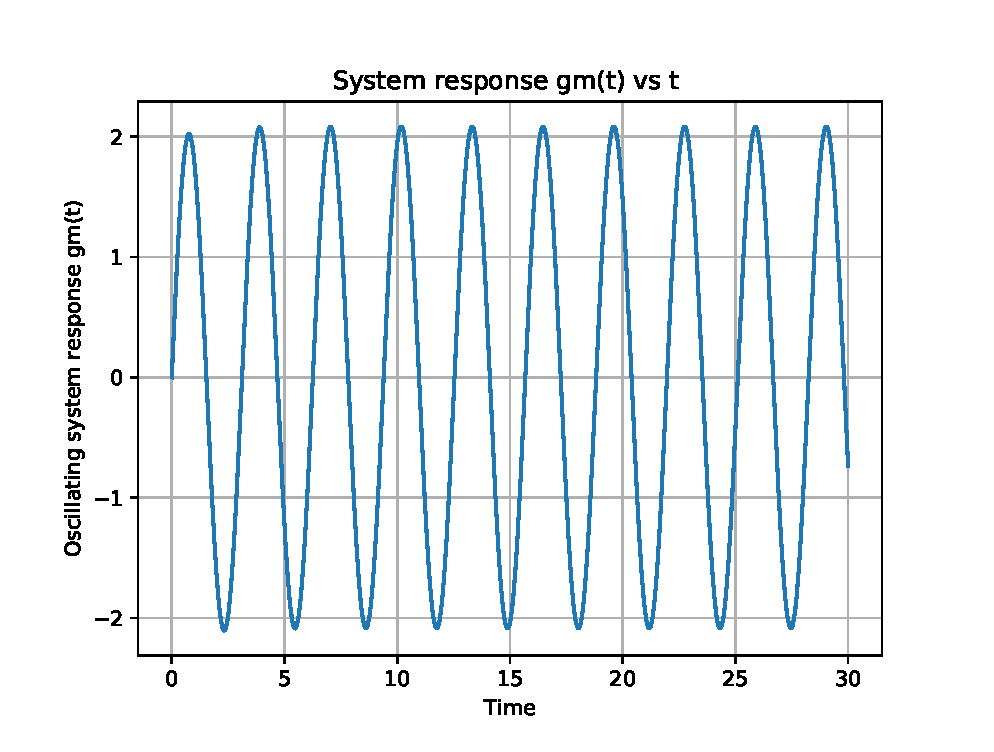
\includegraphics[width=\columnwidth]{Figure_1.eps}
 
\end{figure}

This shows that system oscillates at 2 rad/sec.
\end{enumerate}
